\chapter{Fundamente teoretice}\label{ch:3fundamenteTeoretice}

	În acest capitol voi prezenta principalele concepte teoretice utilizate în realizarea proiectului, împreună cu mediile de dezvoltare, limbajele de programare și framework-urile folosite. 

\section{Medii de dezvoltare}

\subsection{Arduino IDE}

	Pentru programarea plăcuțelor Arduino, se folosește un mediu de dezvoltare numit Arduino Integrated Development Environment. Acesta suportă limbajele de programare C si C++ \cite{arduinoIDE}. 

	Poate rula pe mai multe platforme precum: Windows, Linux, MAC și Java \cite{arduinoIDE}. De asemenea, este important de menționat faptul că este compatibil cu o serie largă de modele de plăcuțe, câteva exemple fiind \cite{arduinoIDE}:
		\begin{itemize}
			\setlength{\itemindent}{2em}
			\itemsep0em
			\item Arduino Uno
			\item Arduino Mega
			\item Arduino Leonardo
			\item Arduino Micro
		\end{itemize} 

	Arduino IDE îndeplinește atât rolul de editor de text, cât și rolul de compilator. Editorul de text reprezintă un suport pentru redactarea codului, iar compilatorul este responsabil de transformarea codului sursă în cod obiect și încărcarea acestuia pe microcontroler \cite{arduinoIDE}.

\subsection{PyCharm}

	Acesta este un mediu de dezvoltare dedicat limbajului de programare \textit{Python}. Prezintă o serie de funcționalități ce facilitează programarea în acest limbaj. Conform \cite{pyCharm}, caracteristicile esențiale oferite de \textit{PyCharm} sunt:
	\begin{itemize}
		\setlength{\itemindent}{2em}
		\itemsep0em
		\item Completare automată de cod.
		\item Refactorizare rapidă și sigură de cod.
		\item Posibilitatea de a crea teste și de a le rula utilizând interfața cu utilizatorul pusă la dispoziție. 
	\end{itemize}
	
\section{Limbaje de programare}

\subsection{Python}

	Python este un limbaj de programare ce a apărut în anul 1991, fiind realizat de către Guido van Rossum \cite{python}. Se bucură de o evoluție fulminantă, ajungând să fie unul din cele mai utilizate limbaje de programare în anul 2020. Creșterea numărului de programatori care aleg să folosească Python, este datorată  caracteristicilor precum \cite{python}: 
	\begin{itemize}
	\setlength{\itemindent}{2em}
	\itemsep0em
	\item Flexibilitatea, poate fi utilizat într-un număr vast de domenii, de la programare web, până la programare pe plăcuțe. Funcționează pe o multitudine de platforme, printre care se enumeră: Windows, Mac, Linux și Raspberry Pi. 
	\item În ceea ce privește sintaxa acestui limbaj de programare, este una simplă, care permite scrierea de programe utilizând un număr mai mic de linii de cod. 
	\item Poate fi folosit atât pentru programare procedurală, funcțională, dar și orientată pe obiecte.
	\end{itemize}

\subsection{C++}

	C++ este un limbaj de programare bazat pe C. Motivele pentru care creatorul acestui limbaj de programare, Bjarne Stroustrup, a decis să folosească limbajul C ca punct de plecare sunt: flexibilitatea si faptul că este un limbaj apropiat de partea hardware, rulează pe multe platforme și se potrivește cu mediul de programare UNIX \cite{c++}.

	Ceea ce aduce nou este posibilitatea de a programa orientat pe obiecte, o programare de tip generic și face posibil conceptul de abstractizare al datelor \cite{c++}. Numărul de domenii în care C++ poate fi aplicat crește considerabil datorită introducerii noțunii de programare orientată pe obiecte. Aceasta implică modelarea unor entități din lumea reală, și interacțiunile acestora, prin intermediul claselor. 

\subsection{HTML}

	Acesta este un limbaj de programare utilizat pentru a forma interfața aplicației web din punct de vedere structural. Permite impărțirea paginilor în mai multe secțiuni și crearea unor serii de elemente esențiale utilizate în astfel de aplicații, precum: butoane, tabele, formulare, câmpuri de intrare și multe altele. Mai mult decât atât, oferă și posibilitatea formatării de text.  


\section{Plarforme cloud}

\subsection{Heroku}

	Este o platformă cloud ce permite găzduirea aplicațiilor web realizate în diverse limbaje de programare: Ruby, Java, Node.js, Clojure, Scala, Python și PHP \cite{heroku}. După ce aplicația a fost găzduită, aceasta poate fi administrată prin intermediul liniei de comandă pusă la dispoziție de platformă \cite{heroku}.

\subsection{Firebase Realtime Database}

	Este o bază de date găzduită pe cloud, iar informațiile sunt stocate în format JSON \cite{firebase}. De asemenea, nu necesită interogări de tip SQL pentru a stoca sau a citi date și oferă siguranța faptului că datele nu se vor pierde dacă este întreruptă conexiunea \cite{firebase}.

\section{Framework-uri}

\subsection{Flask}

	Este un framework construit pe baza limbajului de programare Python, ce oferă posibilitatea de a dezvolta aplicații web. Faptul că este proiectat ca să fie extins, oferă posibilitatea programatorului de a avea control total asupra aplicației pe care o creează. Prezintă un nucleu robust, care include toate funcționalitățile de bază pe care o aplicație web le necesită, nucleu ce poate fi extins de diverse părți terțe \cite{flask}.

	Pentru a crea aplicații web complexe, utilizarea doar a framework-ului nu este suficientă. Motiv pentru care, flask permite îmbinarea cu limbaje de programare precum javascript, CSS și HTML.

\subsection{Bootstrap}

	Framework utilizat pentru a crea partea de interfață cu utilizatorul, ce combină \textit{HTML}, \textit{CSS} și \textit{JavaScript} \cite{bootstrap}. Prezintă o serie de formulare, meniuri de navigare și multe alte elemente de aspect predefinite.  


\section{Componente utilizate}

\subsection{ESP8266}

	NodeMCU ESP8266 este o placă ce se poate conecta prin WiFi la o rețea de internet. Prezintă o antenă esp8266 ce acceptă standardele 802.11b/g/n și protocolul de securitate WPA/WPA2 \cite{esp8266}. Integrează un modul ADC pe 10 biți, microcontroler pe 32 de biți, ce are un consum redus de energie, și se bazează pe protocolul TCP/IP pentru a face transferul de date \cite{esp8266}.

\subsection{Placă de bază pentru NodeMCU}

	Are rolul de a alimenta modulul wireless ESP8266 și de a oferi o extensie pentru pinii pe care acesta îi pune la dispoziție. In ceea ce privește alimentarea, se face printr-un conector de tip jack și acceptă valori între 6 și 24 de volți. De asemenea, placa de bază integrează un regulator de tensiune ce convertește valoarea tensiunii de intrare la 5 volți.

\subsection{Arduino Uno}

	Arduino aduce pe piață o serie de plăcuțe cu microcontroler, ce pot fi programate pentru diverse aplicații. De asemenea, bibliotecile puse la dispoziție pentru acest tip de sisteme sunt menite să faciliteze procesul de programare al acestora \cite{arduino}.

	Programarea plăcuței se face prin intermediul conectorului USB. Aceasta prezintă și un conector separat pentru alimentare care suportă tensiuni în intervalul 7 - 12 volți \cite{arduino}, tensiuni ce vor trece prin regulatorul de tensiune integrat în plăcuță.

	În ceea ce privește pinii prezenți pe placa Arduino Uno, există 6 intrări analogice \cite{arduino}, 14 terminale care pot fi configurate fie ca intrări, fie ca ieșiri \cite{arduino} și o serie de pini ce furnizează tensiune, 3.3 sau 5 volți.

\subsection{LCD 1602}

	Oferă posibilitatea de a afișa text pe două rânduri, fiecare rând conținând 16 caractere. Transferul de date se face prin protocolul $I^2C$, fapt ce reduce considerabil numărul de pini necesari pentru a conecta LCD-ul la Arduino \cite{lcd}.

\vspace{1em}

	Printre caracteristici se remarcă \cite{lcd}:
 		\begin{itemize}
			\setlength{\itemindent}{2em}
			\itemsep0em
			\item Tensiune de alimentare: 5 volți 
			\item Luminozitatea ecranului se poate regla printr-un potențiometru integrat
		\end{itemize} 
	
\subsection{Senzor DHT11}

	Prezintă două părți componente. Prima componentă are rolul de a citi umiditatea ambientală. Este alcatuită din doi electrozi care se suprapun peste un substrat. În momentul în care umiditatea substratului se modifică, determină o modificare a rezistenței dintre cei doi electrozi, iar microcontrolerul detectează și interpretează această valoare. Componenta termică este formată dintr-un termistor. Termistorul este un rezistor a cărui rezistența este invers proporțională cu variația temperaturii. Pe baza valorii rezistenței date de termistor, se vor face prelucrări ajungându-se la o valoare validă a temperaturii.

\subsection{Modul radio frecvență}

	Pereche formată dintr-un transmițător și receptor. Construite pentru a facilita transferul de date prin radio-frecvență. Acestea funcționează la o frecvență de 433Mhz \cite{rfModule}, iar distanța de transmisie diferă în funcție de tensiunea de alimentare a transmițătorului și de calitatea antenelor.

	Conform \cite{rfModule}, se pot evidenția următoarele caracteristici:
 		\begin{itemize}
			\setlength{\itemindent}{2em}
			\itemsep0em
			\item Distanța de transfer: 20 - 200 metri
			\item Tensiune de alimentare transmițător: 3.5 - 12 volți
			\item Rată de transfer: 4 KB/S
			\item Tensiune de alimentare a receptorului: 5 volți
		\end{itemize} 

\subsection{Releu}

	Funcționează ca un întrerupător într-un circuit electric. Principiul de bază al unui releu constă în alăturarea unui solenoid și a unor contacte metalice. În momentul în care solenoidul este alimentat, acesta produce un câmp electromagnetic ce va acționa contactele metalice, deschizând sau închizând circuitul. Releele pe care le utilizez funcționează la 5 volți și au o structură puțin mai complexă, structură pe care intenționez să o detaliez. Prezintă trei intrări: VCC, GND și IN, unde pinii de VCC si GND sunt alimentați permanent, iar IN este pinul de semnal. Acesta este legat la baza unui tranzistor, iar în funcție de tensiunea pe care o furnizează, tranzistorul trece în regim saturat sau blocat, funcționând ca un întrerupător pentru solenoid. De asemenea, în paralel cu bobina este montată o diodă ce are ca și scop protejarea tranzistorului de șocurile de tensiune ce pot apărea la deconectarea alimentării bobinei. Este necesară utilizarea releului pentru a putea controla, prin semnale de putere mică, dispozitive ce funcționează la tensiuni și curenți mari. 

\subsection{Electrovalvă}

	Este un mecanism ce are ca rol deschiderea circuitului de apă în momentul în care este conectat la o sursă de tensiune. Acesta este format dintr-un solenoid și un obturator. Electrovalvele pe care le folosesc sunt de tip normal închis, ceea ce înseamnă că atunci când solenoidul nu este alimentat, obturatorul stă în poziție închis, iar circuitul de apă prin electrovalvă este blocat. În momentul alimentării solenoidului, câmpul magnetic produs de acesta va acționa obturatorul, făcând posibilă trecerea apei prin electrovalvă.

\subsection{Pompă de apă}

	Este alcătuită dintr-un motor electric ce funcționează la 12 volți, curent continuu și acționează o paletă ce pune în mișcare apa din circuit.   

\subsection{Push buton}

	Este un intrerupător, fără reținere, ce are rolul de a trimite semnale către microcontroler. Prezintă două contacte metalice care închid circuitul în momentul în care se ating. 

\subsection{Condensator}

	Este o componentă electrică pasivă ce are rolul de a înmagazina tensiune. Acesta se utilizează în circuitele electrice pentru a reduce fluctuațiile de tensiune ce pot apărea.

\subsection{Rezistență}

	Asemenea condensatorului, rezistența se încadrează în categoria componentelor electrice pasive. Aceasta are rolul de a se opune trecerii curentului electric. 

\subsection{Circuit integrat Schmitt-Trigger}

	Acesta este utilizat pentru a transforma un semnal analog într-un semnal digital, dar prezintă și rolul de inversor. Dacă se aplică la intrare un semnal cu nivel logic 1, la ieșirea din circuitul integrat va avea nivelul logic 0.

\subsection{Diodă}

	Limitează trecerea curentului electric într-un singur sens, de la anod la catod. Prezintă multe utiliăți în circuitele electrice, un exemplu practic fiind conversia curentului alternativ în curent continuu. 

\section{Filtrarea semnalelor}

	Butoanele pe care le-am folosit, pentru setarea temperaturii dorite, sunt formate din contacte metalice. În momentul în care acestea se ating, produc o vibrație pe care microcontrolerul o percepe ca o apăsare multiplă a butonului. Pentru a rezolva această problemă este necesară crearea unor filtre trece jos \cite{buttonDebouncing} pentru fiecare buton în parte. Rolul acestor filtre este de a permite trecerea semnalelor cu frecvență mică si de a opri semnalele cu frecvențe mari. Pentru aceasta, am utilizat circuite RC serie, iar valorile rezistenței si condesatorului au fost calculate utilizând ecuația de încărcare și de descărcare a condensatorului. De asemenea, pentru a obține o filtrare cât mai bună, am utilizat un circuit integrat Schmitt-Trigger. Caracteristica datorită căreia acesta îmbunătățește filtrarea semnalului este histereza pe care o are între pragul superior, declanșează trecerea pe nivel logic 0, și pragul inferior, declanșează trecerea pe nivel logic 1.  
\vspace{1em}\\
Conform \cite{buttonDebouncing}, ecuația de încărcare a condensatorului este:

\begin{equation}
V_{cap} = V_{in}(1-e^{\frac{-t}{RC}})
\end{equation}
\vspace{1em}\\
Conform \cite{buttonDebouncing}, ecuația de descărcare a condensatorului este:

\begin{equation}
V_{cap} = V_{in}(e^{\frac{-t}{RC}})                 
\end{equation}
\vspace{1em}\\
$V_{cap}$ - tensiunea stocată în condensator la momentul t
\vspace{0.7em}\\
$V_{in}$ - tensiune de alimentare a circuitului
\vspace{0.7em}\\
t - timpul măsurat din momentul aplicării tensiunii de alimentare la bornele circuitului, în cazul ecuației de încărcare a condensatorului. Pentru ecuația de descărcare a condensatorului, reprezintă timpul măsurat din momentul întreruperii alimentării circuitului
\vspace{0.7em}\\
R - valoarea în ohmi a rezistenței utilizate
\vspace{0.7em}\\
C - valoarea în farazi a condensatorului utilizat\\ 

\vspace{1em}
	În continuare, pentru a putea aplica formulele, este necesară aflarea timpului cât durează oscilația semnalului. Pentru aceasta, am utilizat un osciloscop ce permite analiza semnalului provenit de la buton.

\begin{figure}[H]
	\centering
    	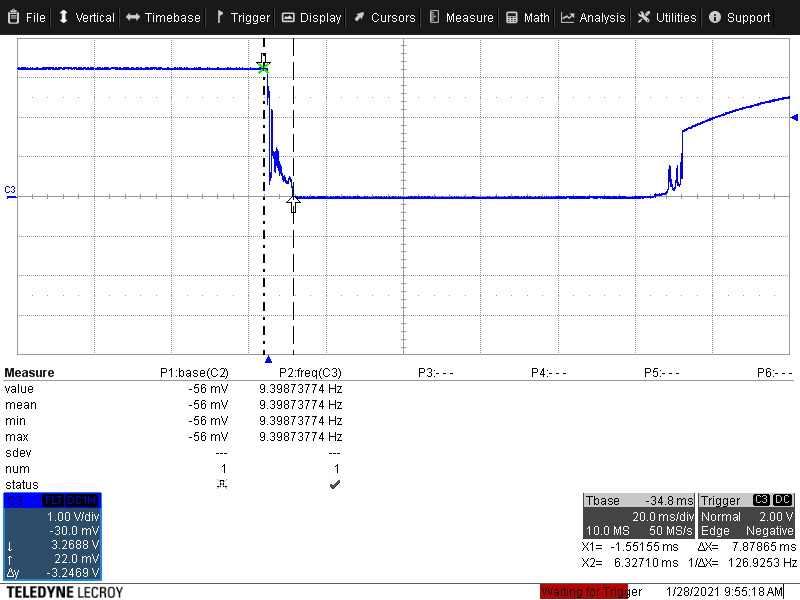
\includegraphics[width=0.8\textwidth]{InainteDeFiltru.jpg}
	\caption{Semnal înainte de filtrul trece jos}
	\label{fig:InainteDeFiltru}
\end{figure}

\begin{figure}[H]
   	\centering
    	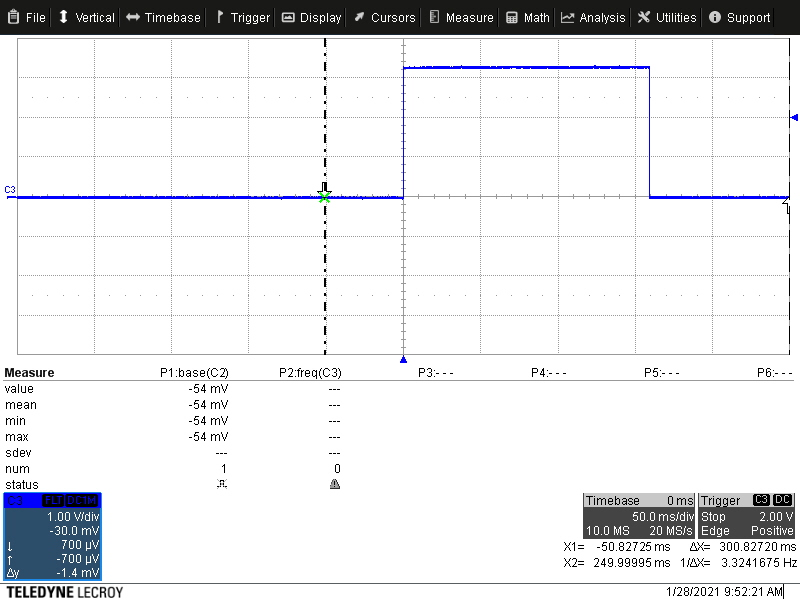
\includegraphics[width=0.8\textwidth]{DupaFiltru.jpg}
	\caption{Semnal după filtrul trece jos}
	\label{fig:DupaFiltru}
\end{figure}
	
	În urma analizei mai multor semnale de la push buton, cea mai mare perturbație a durat aproximativ 8 ms. În calculul valorii rezistențelor si condensatorului care trebuie folosite în filtrele trece jos, voi folosi un timp de 10 ms. Cele 2 ms în plus reprezintă o marjă de siguranță pentru situațiile în care apar perturbații mai mari decât cele măsurate. 

\vspace{1em}

	În cele ce urmează, voi prezenta schema filtrului trece jos, iar pe baza acesteia voi detalia calculele realizate pentru a determina valorile componentelor electrice utilizate.

\begin{figure}[H]
   	\centering
    	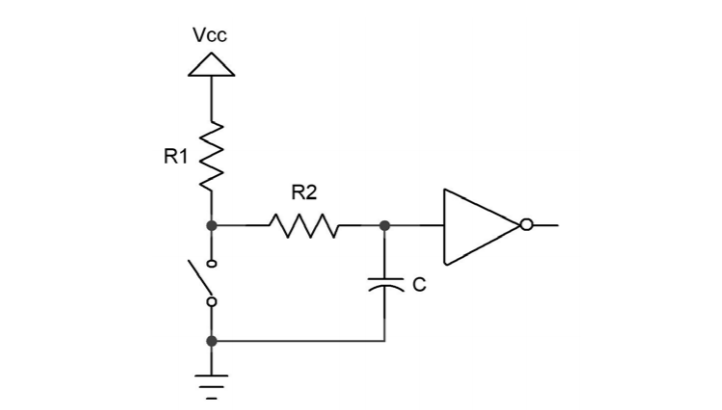
\includegraphics[width=0.8\textwidth]{CircuitRC.png}
	\caption{Schemă filtru trece-jos (sursa: \cite{buttonDebouncing})}
\end{figure}

	În momentul în care întrerupătorul se închide, condensatorul începe să se descarce prin intermediul rezistenței $R_2$. Cunoscând acest aspect, voi putea calcula valoarea $R_2$ utilizând ecuația de descărcare a condensatorului. Valoarea lui t va fi de 10 ms, $V_{in}$ este echivalent cu 3.3 volți(tensiunea la care funcționează modulul WiFi), $V_{cap}$ este egal cu valoarea pragului inferior al inversorului Schmitt-Trigger, iar valoarea condensatorului o aleg de 1 µF. Mai exact, se calculează rezistența astfel încât, după t = 10 ms de la începerea descărcării, tensiunea stocată în condensator să ajungă la valoarea de prag a circuitului integrat.

\[
	R_2 = \frac{-t}{C\ln(\frac{V_{cap}}{V_{in}})} = \frac{-10 \cdot 10^{-3}}{10^{-6}\ln(\frac{1}{3.3})} = \frac{-10}{\ln(0.3)}\cdot 10^3 =  \frac{-10}{-1.2}\cdot 10^3 = 8.33 \cdot 10^3 = 8.33 K\Omega
\]

	Când se deschide întrerupătorul, condensatorul începe să se încarce prin intermediul rezistențelor $R_1$ și $R_2$. Pornind de la această informație, voi calcula valoarea $R_1 + R_2$ utilizând ecuația de încărcare a condensatorului. Doar valoarea parametrului $V_{cap}$ se modifică, va fi echivalentă cu pragul superior al inversorului. 

\[
	R_1 + R_2 = \frac{-t}{C\ln(1 - \frac{V_{cap}}{V_{in}})} = \frac{-10 \cdot 10^{-3}}{10^{-6}\ln(1 - \frac{1.5}{3.3})} = \frac{-10}{\ln(0.54)}\cdot 10^3 =  \frac{-10}{-0.61}\cdot 10^3 = 16.39 \cdot 10^3
\]
\[
	 = 16.39 K\Omega
\]
\[
	R_1 + R_2 = 16.39 K\Omega, R_2 = 8.33 K\Omega \Rightarrow R_1 = 8.06 K\Omega
\]	
	
\section{Histereza}

	Pentru a evita crearea unui lanț de porniri si opriri repetate, pe perioade scurte de timp, cauzate de fluctuațiile rapide de temperatură, este necesară implementarea conceptului de histereză. Acesta constă în stabilirea unei valori de toleranță la temperatura setată, astfel încât diferența de temperatură din momentul în care se trimite comandă pentru oprirea sistemului de încălzire, până la următoarea pornire a acestuia, să fie egală cu dublul valorii histerezei. Cu alte cuvinte, comanda de pornire a încalzirii se va da când temperatura în cameră ajunge să fie mai mică sau egală cu valoare temperaturii setate, din care se sustrage valoarea histerezei, iar comanda de oprire va fi declanșată când temperatura ambientală este mai mare sau egală cu valoarea temperaturii setate, la care se adaugă valoare histerezei. În acest fel, timpul între comenzi este mai mare și numărul de cicluri pornit/oprit este mai mic, măsură ce este menită să protejeze sistemele de încălzire.


	 
 